\documentclass[a4paper,11pt]{article}

\usepackage[T1]{fontenc}
\usepackage[utf8]{inputenc}
\usepackage{graphicx}
\usepackage{xcolor}
\usepackage{placeins}

\renewcommand\familydefault{\sfdefault}
\usepackage{tgheros}

\usepackage{amsmath,amssymb,amsthm,textcomp}
\usepackage{enumerate}
\usepackage{multicol}
\usepackage{tikz}
\usepackage{float}

\usepackage{geometry}
\geometry{left=25mm,right=25mm,%
bindingoffset=0mm, top=20mm,bottom=20mm}


\linespread{1.3}

\newcommand{\linia}{\rule{\linewidth}{0.5pt}}

% custom theorems if needed
\newtheoremstyle{mytheor}
    {1ex}{1ex}{\normalfont}{0pt}{\scshape}{.}{1ex}
    {{\thmname{#1 }}{\thmnumber{#2}}{\thmnote{ (#3)}}}

\theoremstyle{mytheor}
\newtheorem{defi}{Definition}

% my own titles
\makeatletter
\renewcommand{\maketitle}{
\begin{center}
\vspace{2ex}
{\huge \textsc{\@title}}
\vspace{1ex}
\\
\linia\\
\@author \hfill \@date
\vspace{4ex}
\end{center}
}
\makeatother
%%%

% custom footers and headers
\usepackage{fancyhdr}
\pagestyle{fancy}
\lhead{}
\chead{}
\rhead{}
\lfoot{}
\cfoot{}
\rfoot{\thepage}
\renewcommand{\headrulewidth}{0pt}
\renewcommand{\footrulewidth}{0pt}
%

% code listing settings
\usepackage{listings}
\lstset{
    language=Python,
    basicstyle=\ttfamily\small,
    aboveskip={1.0\baselineskip},
    belowskip={1.0\baselineskip},
    columns=fixed,
    extendedchars=true,
    breaklines=true,
    tabsize=4,
    prebreak=\raisebox{0ex}[0ex][0ex]{\ensuremath{\hookleftarrow}},
    frame=lines,
    showtabs=false,
    showspaces=false,
    showstringspaces=false,
    keywordstyle=\color[rgb]{0.627,0.126,0.941},
    commentstyle=\color[rgb]{0.133,0.545,0.133},
    stringstyle=\color[rgb]{01,0,0},
    numbers=left,
    numberstyle=\small,
    stepnumber=1,
    numbersep=10pt,
    captionpos=t,
    escapeinside={\%*}{*)}
}

%%%----------%%%----------%%%----------%%%----------%%%

\begin{document}

\title{CS 426 Parallel Computing Project 4 Report}

\author{Bartu Atabek - 21602229}

\date{29/05/2020}

\maketitle

\section{Answers to The Questions}
\subsection{What is control flow divergence?}

Flow divergence also known as the warp divergence, is meant for a performance issue while in kernel functions, if we meet a conditional branch like if, different threads of the current warp can enter different sections of the branch which damages the parallelism since it is wanted for warps to act parallel. If different threads go in the same branch, it is very efficient otherwise, performance decreases significantly.

\subsection{How can we create a dynamic sized shared memory?}

Creating dynamic sized memory is similar to creating static sized memory but it has little differences. While creating dynamic sized memory, we put at the start of the initialization line \textbf{extern} keyword, then  \textbf{\_\_shared\_\_}, then the type of the memory and then name of it. Below line holds an example declaration.
\newline
\newline
Example: \textbf{extern \_\_shared\_\_ float shared\_data[]}
\newline
\newline
We do not specify the size of it, as it is dynamic We can use as much as space that the caller passed as parameter to global function. It is passed as the third argument of the \textbf{"< < <  > > >"} block

\subsection{How can we use shared memory to accelerate our code?}

The shared memory is much faster than the global memory as it is just on the same chip GPU resides. It is almost 100 times faster than the global memory. Shared memory is spared for all the threads in current function. They all can read and write to it so we should be careful while using it. As it is faster, we should use it but we should be using it in a safe way. For example, two threads should not update the same location at the same time or one should not read the location while other one is writing at the same time. These kinds of issues can be handles in some ways in CUDA. One of them is to use atomic operations like atomicadd and atomicsub.

\subsection{Which CUDA operations give us device properties? To answer this question you should
write a simple program and query the device properties of the machine you are working
with.}

In CUDA, there is a data structure which is called, cudaDeviceProp, it can be initialized with the function cudaGetDeviceProperties. After then, we can easily obtain the information about our CUDA device as we want. For example, after initialization of cudaDeviceProp, we can obtain our devices total global memory as prop.totalGlobalMem or we can learn maximum threads per block as pro.maxThreadsPerBlock

\subsection{What are the necessary compiler options in order to use atomic operations?}

In CUDA, to use atomic operations, our compiled binary architecture should match the device architecture. To check this, we should look at our device architecture code from NVDIA website or
from device properties. This architecture type should match the one in the Project properties > C/C++ > Device > Code Generation > compute.....

\section{Results \& Discussion}
\subsection{Implementation Details}

In my implementation, I firstly do the basic things of every CUDA program. Allocated memory for host variables and kernel variables, memcpy my host variables to kernel ones. Then I call the \textbf{\_\_global\_\_}function to execute my kernel code. I passed 4 parameters to it, the first two ones are the 2 vector arrays. I create them in the function arrayGenerator before calling the \textbf{\_\_global\_\_} func. I pass N to my array generator function and it returns me a 2 arrays which have size of N and every member of them has a random value between 0 and 100. In my \textbf{\_\_global\_\_} function, I basically applied the very similar approach to find firstly, the doc product of the 2 vectors, then, their individual, length by summing up their values to the power of 2 and then square rooting at the end. I output 3 values from this function, dot product,sum of power 2 of each vector. This was enough. Then, I divide the dot product into the multiplication of sqrt of each vector’s length. In my CPU function, I again find firstly the dot product of two vectors and their individual power 2 and sqrt of them and their division.

\subsection{Results as Plots}

\begin{figure}[!htb]
    \centering
    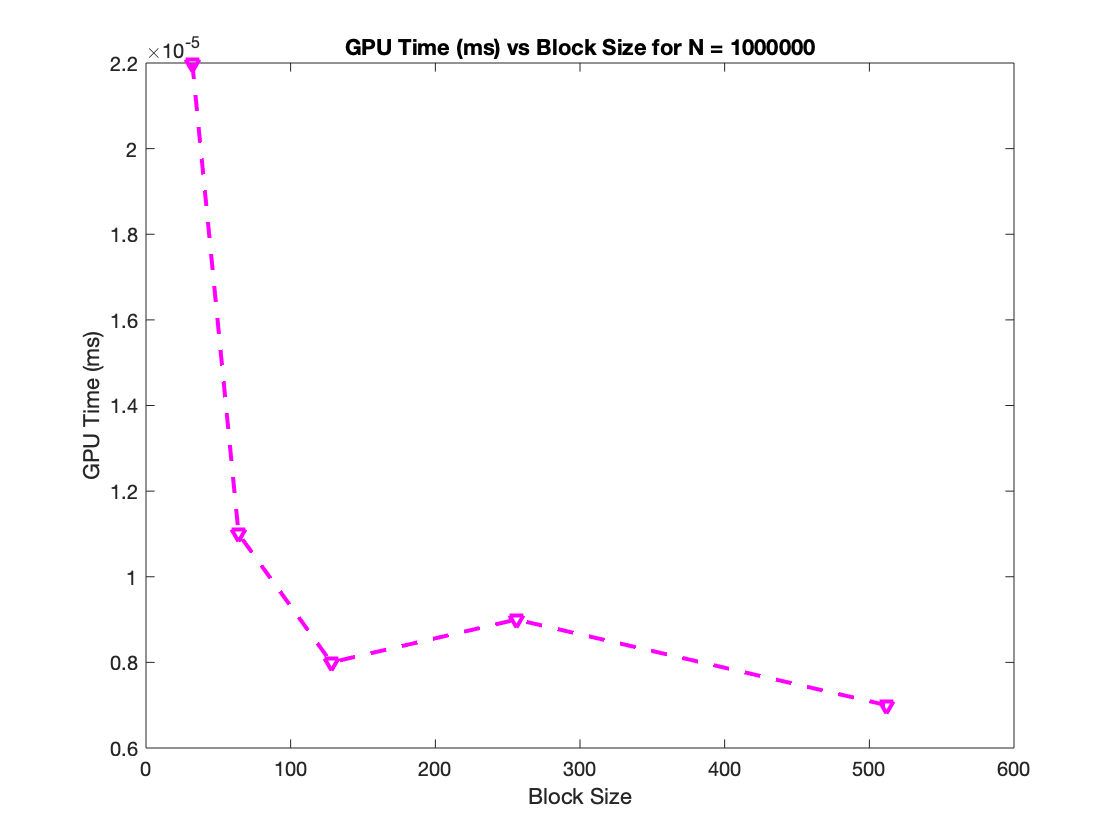
\includegraphics[width=0.75\textwidth]{figure1}
    \caption{When N is constant as 1000000 and blocksize is 32, 64, 128, 256, 512. Time in nanoseconds}
\end{figure}
\FloatBarrier
\begin{figure}[!htb]
    \centering
    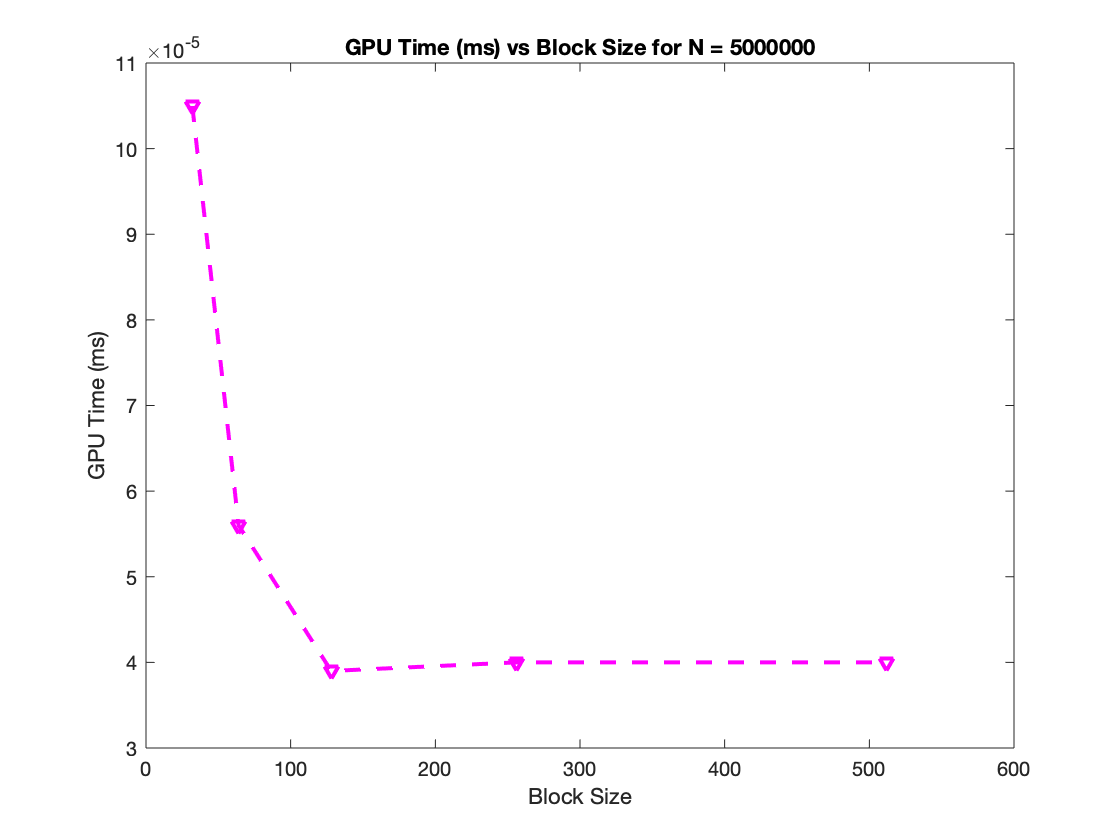
\includegraphics[width=0.75\textwidth]{figure2}
    \caption{When N is constant as 5000000 and blocksize is 32, 64, 128, 256, 512. Time in nanoseconds}
\end{figure}

% \makeatletter
% \setlength{\@fptop}{0pt}
% \makeatother
\begin{figure}[!htb]
    \centering
    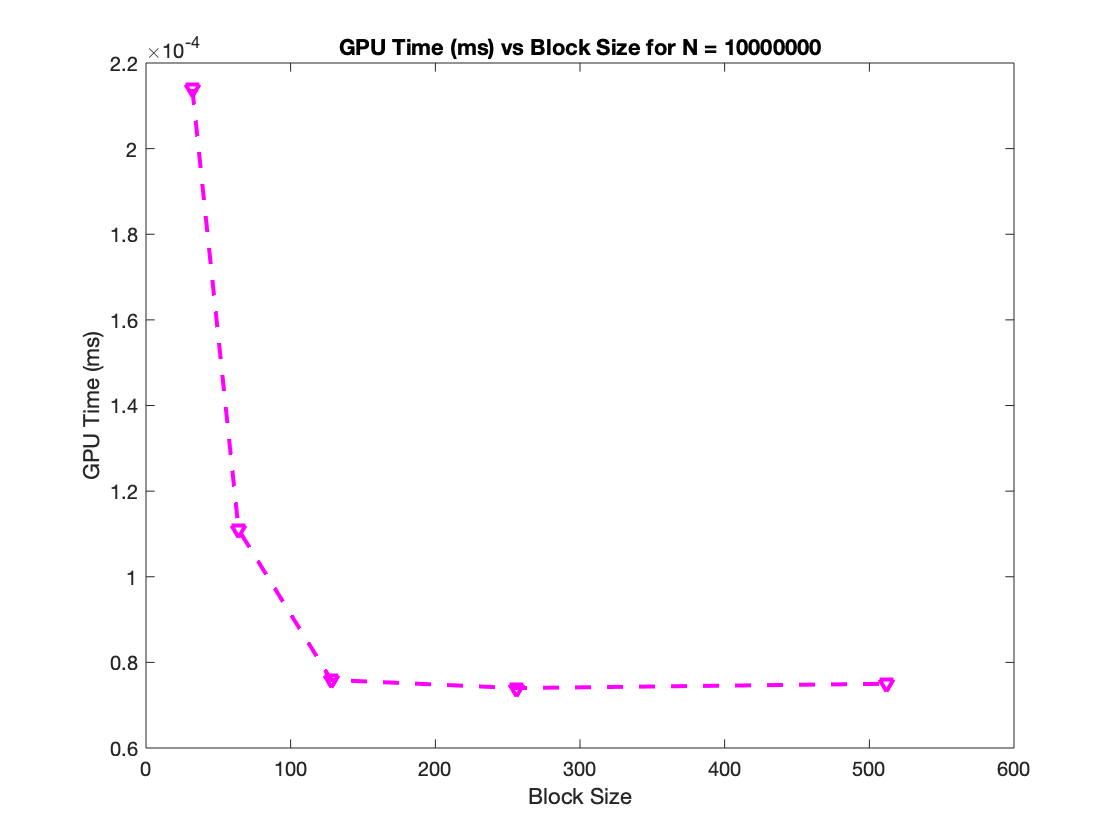
\includegraphics[width=0.75\textwidth]{figure3}
    \caption{When N is constant as 10000000 and blocksize is 32, 64, 128, 256, 512. Time in nanoseconds}
\end{figure}

\FloatBarrier
\subsection{Discussion of Results}

In the project, as it can be seen in graphs, the elapsed time for GPU is decreased when the block size increased. However; after some point, after 128, increase in number of blocks did not affect the elapsed time much, it may be because of the fact that we reached an almost upperlimit for increase because while going from 32 to 64 and 64 to 128, decrease was very high but then it almost stopped. Also, when the size of the vector is increase, the time is also increasing. 

As a disclosure I can say that there may be a small index difference between the CPU results and the GPU results. I am not entirely sure the reason behind this because I tried different algorithms and still experienced this problem. I also tried the kernel code in the official Nvidia documentation. I could not solve this as I go over the code and it seems correct.
\end{document}
